\chapter{Моменты случайных величин}

\section{Математические ожидания}

\begin{definition}
	\emph{Математическим ожиданием} случайной величины $ \xi $ называется её усреднённое значение,
	\ie среднее ожидаемое значение функции $ \xi(\omega) $, которое выражается в виде интеграла по
	вероятностной мере
	$$ \mathbb E \xi = \int\limits_\Omega \xi(\omega) P\Set{\di \omega} $$

	Если множество $ \Omega $ состоит из конечного или счётного набора элементарных исходов, то
	$$ \mathbb E \xi = \sum \xi(\omega_i)P(\omega_i) $$

	Для дискретного распределения
	$$ \mathbb E \xi = \sum_k x_k P\Set{\xi = x_k} $$

	Для абсолютно непрерывного распределения
	$$ \mathbb E \xi = \int_{-\infty}^\infty xp_\xi(x) \di x $$
\end{definition}

Если от величины $ \xi $ переходим к величине $ \eta = g(\xi) $, то математическое ожидание можно
выразить через распределение исходной величины:
$$ \mathbb E \eta = \sum_k g(x_k) P \Set{\xi = x_k}, \quad \text{дискретное распределение} $$
$$ \mathbb E \eta = \int_{-\infty}^\infty g(x) p_\xi(x) \di x, \quad \text{абсолютно непрерывное
распределение} $$

\begin{definition}
	Пусть $ g(x) = x^n $.
	$$ \mathbb E \eta = \mathbb E g(\xi) = \mathbb E \xi^n =
	\int_{-\infty}^\infty x^n \di F_\xi(x) =
	\begin{cases}
		\sum x_k^n P\Set{\xi = x_k} \\
		\int x^n p_\xi(x) \di x
	\end{cases} $$

	$ \mathbb E \xi^n $ называется \emph{начальным моментом} случайной величины
	$ \xi $ порядка $ n $.
\end{definition}

\begin{definition}
	Если возьмём $ g(x) = (x - \mathbb E \xi)^n $, то получим
	$ \mathbb E(\xi - \mathbb E \xi)^n $ "--- \emph{центральный момент} порядка $ n $.
\end{definition}

\begin{definition}
	При $ g(x) = |x|^n $ получаем $ \mathbb E|\xi|^n $ "--- \emph{абсолютный начальный момент}
	порядка $ n $.
\end{definition}

\begin{definition}
	Если $ g(x) = |x - \mathbb E \xi|^n $, то получаем $ \mathbb E|\xi - \mathbb E \xi|^n $ "---
	\emph{абсолютный центральный момент} порядка $ n $.
\end{definition}

\begin{definition}
	Второй центральный момент случайной величины $ D \xi = \mathbb E(\xi - \mathbb E \xi)^2 $
	называется \emph{дисперсией} этой случайной величины.
\end{definition}

\subsection{Свойства математических ожиданий}

\begin{props}
\item Если математические ожидания $ \xi $ и $ \eta $ существуют, то
	$ \mathbb E(\xi + \eta) = \mathbb E \xi + \mathbb E \eta $.
\item $ \mathbb E(\alpha + \beta \xi) = \alpha + \beta \mathbb E\xi $.
\item $ \mathbb E c = c $.
\item $ P\Set{\alpha \le \xi \le \beta} = 1 \implies \alpha \le \mathbb E \xi \le \beta $.
\item $ \xi \le \eta \implies \mathbb E \xi \le \mathbb E \eta $.
\item $ |\mathbb E \xi| \le \mathbb E |\xi| $ (\as $ -|\xi| \le \xi \le |\xi| $).
\item Если $ P \Set{\xi \ge 0} = 1 $ и $ \mathbb E \xi = 0 $, то $ P\Set{\xi = 0} = 1 $.
\item Если $ \xi $ и $ \eta $ независимы, то $ \mathbb \xi \eta =
	\mathbb E \xi \cdot \mathbb E \eta $.
\end{props}

\subsection{Свойства дисперсии}

\begin{props}
\item $ D\xi \ge 0 $.
\item Если $ D \xi = 0 $, то $ P\Set{\xi = C} = 1 $ в некоторой точке $ C $.
\item $ D(\alpha \xi + \beta) = \alpha^2 D\xi $.
\item Если $ \xi $ и $ \eta $ независимы, то $ D(\xi \pm \eta) = D\xi + D\eta $.
\item $ D(\xi + \eta) = D\xi + D\eta + 2 \operatorname{cov}(\xi, \eta) $, где
    $ \operatorname{cov}(\xi, \eta) = \mathbb E(\xi \eta) - \mathbb E \xi \mathbb E \eta $.
\item $ D\xi \ge D|\xi| $.
\item $ D \xi = \mathbb E\xi^2 - (\mathbb E \xi)^2 $.
\end{props}

\subsection{Вычисление математических ожиданий и дисперсий}

\begin{enumerate}
	\item \emph{Вырожденное распределение}
		$$ P\Set{\xi = C} = 1 $$
		$$ \mathbb E \xi = C, \quad D\xi = 0 $$
	\item \emph{Двухточечное распределение}
		$$ \xi =
		\begin{cases}
			0 \quad \text{ с вероятностью } q = 1 - p \\
			1 \quad \text{ с вероятностью } p
		\end{cases} $$
		$$ \mathbb E \xi = p, \quad D \xi = p(1 - p) $$
		$$ \eta =
		\begin{cases}
			a \quad \text{ с вероятностью } q = 1 - p \\
			b \quad \text{ с вероятностью } p
		\end{cases} $$
		$$ D \eta = (b - a)^2p(1 - p) $$
	\item \emph{Биномиальное распределение} ($ \xi \sim B(n, p) $)

		$ \xi $ принимает значения $ 0, 1, 2, \dots, n $ с вероятностями
		$$ p_k = C_n^kp^k(1 - p)^{n - k} $$
		$$ \mathbb E \xi = np, \quad D \xi = np(1 - p) $$
	\item \emph{Пуассоновское распределение} ($ \xi \sim \pi(\lambda) $)
		$$ P\Set{\xi = k} = e^{-\lambda}\frac{\lambda^k}{k!} $$
		$$ \mathbb E \xi = \lambda, \quad D\xi = \lambda $$
	\item \emph{Геометрическое распределение} ($ \xi \sim \operatorname{Geom}(p) $)

		$ \xi $ принимает значения $ 0, 1, 2, \dotsc $ с вероятностями
		$$ P_k = (1 - p)p^k $$
		$$ \mathbb E\xi = \frac p{1 - p}, \quad D \xi = \frac p{(1 - p)^2} $$
	\item \emph{Равномерное распределение} ($ \xi \sim U[a, b] $)

		Плотность распределения имеет следующий вид:
		$$ p(x) =
		\begin{cases}
			\frac1{b - a}, \quad x \in [a, b], \\
			0, \quad x \not\in [a, b]
		\end{cases} $$
		$$ \mathbb E \xi = \frac{b + a}2, \quad D \xi = \frac{(b - a)^2}{12} $$
	\item \emph{Экспоненциальное распределение} ($ \xi \sim E(\lambda) $)

		Плотность $ \xi $ имеет вид
		$$ p(x) =
		\begin{cases}
			0, \quad x < 0, \\
			\frac1\lambda e^{-\frac x \lambda}, \quad x \ge 0
		\end{cases} $$
		$$ \mathbb E \xi = \lambda, \quad D\xi = \lambda^2 $$
	\item \emph{Распределение Коши}
		$$ p(x) = \frac1\pi (1 + x^2) $$
		$$ \int\limits_{-\infty}^\infty p(x) \di x = \infty $$
		Значит, математического ожидания и дисперсии $ \xi $ не существует.
		Более того, понятно, что и моментов более высокого порядка не существует.
	\item \emph{Нормальное распределение} ($ \xi \sim N(a, \sigma^2) $)
		$$ p(x) = (2\pi)^{-\frac12} \frac1\sigma e^{-\frac{(x - a)^2}{2\sigma^2}} $$
		$$ \mathbb E \xi = a, \quad D \xi = \sigma^2 $$
\end{enumerate}

\section{Вероятностные неравенства}

\begin{lemma}[Чебышёва]
	$ \xi \ge 0, \quad \exists \mathbb E \xi, \quad t > 0 $

	$$ P\Set{\xi \ge t} \le \frac{\mathbb E \xi}t $$
\end{lemma}

\begin{proof}
	$$ P\Set{\xi \ge t} = \int_t^\infty \di F(x) \le \frac1t \int_t^\infty x \di F(x) \le
	\frac1t \int_0^\infty x \di F(x) = \frac{\mathbb E \xi}t $$
\end{proof}

\begin{remark}
	Аналогично,
	$$ P\Set{\xi \ge t} \le \frac{\mathbb E\xi^2}{t^n} $$
\end{remark}

Подставляя $ \xi = (\xi - \mathbb \xi)^2 $ и $ t = \eps^2 $, получаем следующий результат

\begin{statement}[неравенство Чебышёва]
	$ \exists \mathbb E \xi, ~ D \xi, \quad \eps > 0 $

	$$ P\{|\xi - \mathbb E\xi| > \eps\} \le \frac{D\xi}{\eps^2} $$
\end{statement}

\begin{statement}[неравенство Ляпунова]
	$ \gamma_n \coloneq \mathbb E |\xi|^n $

	$$ \implies \gamma_1 \le \gamma_2^{\frac12} \le \gamma_3^{\frac13} \le \dots \le
	\gamma_{m - 1}^{\frac1{m - 1}} \le \gamma_m^{\frac1m} \le \dotsb $$

	$$ \phi(a) = (\mathbb E|\xi|^\alpha)^{\frac1\alpha} $$

	Тогда $ \phi $ монотонно возрастает.
\end{statement}

\section{Смешанные моменты}

\begin{definition}
	Для $ n $-мерного случайного вектора $ \ol\xi = (\xi_1, \dots, \xi_n) $ рассмотрим
	\emph{математическое ожидание}
	$$ \mathbb E g(\xi_1, \dots, \xi_n) = \iiint\limits_{-\infty}^\infty g(x_1, \dots, x_n)
	F(\di x_1, \dots, \di x_n) $$

	Для дискретных случайных векторов имеем
	$$ \mathbb Eg(\xi_1, \dots, \xi_n) = \sum P\Set{\xi_1 = x_1, \dots, \xi_n = x_n}
	g(x_1, \dots, x_n) $$

	Для абсолютно непрерывных случайных векторов
	$$ \mathbb Eg(\xi_1, \dots, \xi_n) = \iiint\limits_{-\infty}^\infty g(x_1, \dots, x_n)
	p(x_1, \dots, x_n) \di x_1 \dots \di x_n $$
\end{definition}

Пусть $ \xi, \eta $ "--- независимые случайные величины.
Тогда
$$ F_{\xi, \eta}(x, y) = F_\xi(x)F_\eta(y) $$

\begin{statement}
	Если $ g(x, y) = h(x)r(y) $, то
	$$ \mathbb Eg(\xi, \eta) = \mathbb E \bigl( h(\xi)r(\eta) \bigr) =
	\int\limits_{-\infty}^\infty \int\limits_{-\infty}^\infty h(x)r(y) F_{\xi, \eta}(\di x, \di y) =
	\int\limits_{-\infty}^\infty h(x)F_\xi(\di x) \int\limits_{-\infty}^\infty r(y) F_\eta(\di y) =
	\mathbb Eh(\xi) \mathbb E r(\eta) $$
\end{statement}

\begin{definition}
	\emph{Начальный смешанный момент} порядка $ n + m $ определяется для двумерных дискретных и
	двумерных абсолютно непрерывных векторов следующими соотношениями:
	$$ \mathbb E\xi^n \eta^m = \sum_k \sum_l x_k^n y^-l^m P\Set{\xi = x_k, ~ \eta = y_l} $$
	$$ \mathbb E\xi^n\eta^m = \int\limits_{-\infty}^\infty \int\limits_{-\infty}^\infty x^ny^m
	p_{\xi, \eta}(x, y) \di x \di y $$
\end{definition}

\begin{definition}
	Если взять $ g(x, y) = (x - \mathbb E\xi)^n (y - \mathbb E\eta)^m $, то математическое ожидание
	$ \mathbb E(\xi - \mathbb E\xi)^n(\eta - \mathbb E \eta)^m $ называется
	\emph{центральным смешанным моментом} порядка $ n + m $.
\end{definition}

\begin{definition}
	Центральный смешанный момент $ \operatorname{cov}(\xi, \eta) =
	\mathbb E(\xi - \mathbb E\xi)(\eta - \mathbb E \eta) $ называется \emph{ковариацией}.
\end{definition}

\subsection{Свойства ковариаций}

\begin{props}
\item $ \mathbb E(\xi - \mathbb E\xi)(\eta - \mathbb E\eta) =
	\mathbb E(\xi\eta) - \mathbb E\xi \mathbb E \eta $.
\item $ \operatorname{cov}(\xi, \xi) = \mathbb E(\xi - \mathbb E \xi)^2 = D\xi $.
\item $ \operatorname{cov}(\alpha \xi + \beta, \gamma \eta + \delta) =
	\alpha \gamma \operatorname{cov}(\xi ,\eta) $.
\item Если $ \xi $ и $ \eta $ независимы, то $ \operatorname{cov}(\xi, \eta) = 0 $.
\item\label{cov-prop-5} $ |\operatorname{cov}(\xi, \eta)| \le \sqrt{D\xi D\eta} $.
\end{props}

\begin{proof}[\ref{cov-prop-5}]
	$$ D \Bigl( \frac\xi{\sqrt{D\xi}} + \frac\eta{\sqrt{D\eta}} \Bigr) =
	2 + 2 \frac{\operatorname{cov}(\xi, \eta)}{\sqrt{D\xi} \sqrt{D\eta}} \ge 0 $$
	$$ D \Bigl( \frac\xi{\sqrt{D\xi}} - \frac\eta{\sqrt{D\eta}} \Bigr) =
	2 - 2 \frac{\operatorname{cov}(\xi, \eta)}{\sqrt{D\xi} \sqrt{D \eta}} \ge 0 $$
\end{proof}

\subsection{Коэффициент корреляции}

Пусть $ \xi, \eta $ "--- невырожденные случайные величины, у которых существуют дисперсии.
Рассмотрим их центрированные и нормированные варианты
$$ \hat\xi = \frac{\xi - \mathbb E \xi}{\sqrt{D \xi}}, \quad \hat \eta =
\frac{\eta - \mathbb E \eta}{\sqrt{D \eta}} $$

Имеем равенства
$$ \mathbb E \hat \xi = \mathbb E \hat \eta = 0, \quad D \hat \xi = D \hat \eta = 1 $$

\begin{definition}
	\emph{Коэффициент корреляции} $ \rho $ между $ \xi $ и $ \eta $ задаётся равенством
	$$ \rho(\xi, \eta) = \operatorname{cov}(\hat \xi, \hat \eta) =
	\frac{\operatorname{cov}(\xi, \eta)}{\sqrt{D \xi} \sqrt{D \eta}} $$
\end{definition}

\subsection{Свойства коэффициента корреляции}

\begin{props}
\item Если $ \xi, \eta $ независимы, то $ \rho(\xi, \eta) = 0 $.
	В общем случае, если $ \rho(\xi, \eta) = 0 $, то говорим, что $ \xi, \eta $ "---
	\emph{ортогональные (некоррелированные)} случайные величины.
\item $ |\rho| \le 1 $.
\item Если $ |\rho(\xi, \eta)| = 1 $, то $ \eta = \alpha\xi + \beta $, причём
	$ \sign(\rho) = \sign(\alpha) $.
\item $ \rho(\alpha \xi + \beta, \delta \eta + \gamma) = \sign(\alpha \delta) \rho(\xi, \eta) $.
\end{props}

\section{Производящие функции}

\begin{definition}
	$ \Set{a_n \in \mathbb R}_{k = 1}^\infty $
	$$ A(s) = \sum_{n = 0}^\infty a_ns^n $$

	Если ряд сходится на интервале $ [-s_0, s_0], ~ s_0 > 0 $, то функция $ A(s) $ называется
	\emph{производящей функцией} последовательности $ \Set{a_n} $.
\end{definition}

Рассмотрим в качестве $ \Set{a_n} $ распределения вероятностей.
Пусть случайная величина $ \xi $ принимает значения $ 0, 1, \dotsc $ с вероятностями
$ p_n = P\Set{\xi = n} $.

Построим производящую функцию для последовательности $ \Set{p_n} $:
$$ P(s) = \sum_{n = 0}^\infty p_ns^n $$
Ряд сходится абсолютно при $ -1 \le s \le 1 $.
$ P(s) $ "--- производящая функция $ \xi $.
Её можно представить в виде
$$ P(s) = \sum_{n = 0}^\infty p_ns^n = \mathbb Es^\xi $$

\begin{exmpls}
\item Биномиальное распределение $ \xi \sim B(n, p) $.

	Случайная величина принимает значения $ 0, 1, \dots, n $ с вероятностями
	$$ p_m = C_n^m p^m(1 - p)^{n - m} $$
	
	Её производящая функция имеет вид
	$$ P(s) = \sum_{m = 0}^n C_n^M p^m(1 - p)^{n - m}s^m =
	\sum_{m = 0}^n C_n^m (ps)^m (1 - p)^{n - m} = (1 - p + ps)^n $$
\item Пуассоновское распределение $ \xi \sim \pi(\lambda) $.

	Случайная величина принимает значения $ 0, 1, \dotsc $ с вероятностями
	$$ p_n = e^{-\lambda} \frac{\lambda^n}{n!} $$
	$$ P(s) = \sum_{n = 0}^\infty e^{-\lambda} \frac{(\lambda s)^n}{n!} =
	e^{-\lambda}e^{\lambda s} = e^{\lambda (s - 1)} $$
\item Геометрическое распределение
	$$ p_n = (1 - p)p^n, \quad n = 0, 1, \dots, \quad 0 < p < 1 $$
	$$ P(s) = \sum_{n = 0}^\infty (1 - p)(ps)^n = \frac{1 - p}{1 - ps} $$
\end{exmpls}

\subsection{Свойства производящих функций}

\begin{props}
\item $ P(1) = 1 $.
\item $ |P(s)| \le 1, \quad |s| \le 1 $.
\item Если $ \xi $ и $ \eta $ независимы
    $$ P_{\xi + \eta}(s) = \mathbb Es^{\xi + \eta} =
    \mathbb E s^\xi \cdot \mathbb E s^\eta = P_\xi(s)P_\eta(s) $$
\item $ 0 \le 1 $
	$$ P_\xi(s) = \sum_{n = 0}^\infty p_ns^n \ge 0 $$
	$$ \nder[k]P(s) = \sum_{n = 0}^\infty n (n - 1) \cdots (n - k + 1)p_ns^{n - k} $$
	$$ 0 \le \nder[k]P(s) \le \sum_{n = 0}^\infty n(n - 1) \cdots (n - k + 1)s^{n - k} $$
\item Если известна производящая функция, то можно восстановить вероятности:
	$$ \nder[k]P(0) = k!p_k $$
	$$ p_k = \frac{\nder[k]P(0)}{k!}, \quad p_0 = P(0) $$
\item $ P'(1) = \mathbb E \xi = \sum k p_k $

	Наряду с вероятностями $ p_k = P\Set{\xi = k} $ рассмотрим вероятности $ q_n = P\Set{\xi > n} $.
	\begin{multline*}
		Q(s) = \sum_{n = 0}^\infty q_ns^n =
		\sum_{n = 0}^\infty \Bigl( \sum_{k = n + 1}^\infty p_k \Bigr) s^n =
		\sum_{k = 1}^\infty p_k \sum_{n = 0}^{k - 1}s^n =
		\sum_{k = 1}^\infty p_k \cdot \frac{1 - s^k}{1 - s} = \\
		= \frac1{1 - s} \Bigl( \sum_{k = 1}^\infty p_k - \sum_{k = 1}^\infty p_ks^k \Bigr) =
		\frac1{1 - s} \bigl( 1 - P(s) \bigr)
	\end{multline*}

	При этом,
	$$ Q(s) = \frac{1 - P(s)}{1 - s} $$
	Переходя к пределу по $ s $, получаем
	$$ \lim\limits_{s \to 1} Q(s) = P'(1) = \mathbb E \xi $$

	Отсюда, в частности,
	$$ \mathbb E \xi = \sum_{n = 0}^\infty P\Set{\xi > n} $$
\end{props}

\section{Факториальные моменты}

\begin{definition}
	\emph{Факториальным моментом} порядка $ k $ случайной величины $ \xi $ называется величина
	$$ \mu_k = \mathbb E \bigl( \xi (\xi - 1)(\xi - 2) \cdots (\xi - k + 1) \bigr) $$
\end{definition}

По начальным моментам однозначно находятся факториальные моменты:
$$ \mu_1 = \mathbb E \xi = \alpha_1 $$
$$ \mu_2 = \mathbb E \xi (\xi - 1) = \alpha_2 - \alpha_1 $$
$$ \mu_3 = \mathbb E \xi (\xi - 1) (\xi - 2) = \alpha_3 - 3\alpha_2 + 2\alpha_1 $$

$$ \nder[k]P(s) = \sum_{n = 0}^\infty n (n - 1) \cdots (n - k + 1) p_ns^{n - k}, \quad 0 \le s < 1 $$
Так как $ P(s) $ и её производные "--- монотонные непрерывные функции,
$$ \exists \lim\limits_{s \to 1^-} \nder[k]P(s) = \nder[k]P(1) =
\sum_{n = 0}^\infty n (n - 1) \cdots (n - k + 1)p_n = \mu_k $$

Будем говорить, что существует \emph{конечный факториальный момент}, если существует конечный левый
предел $ \nder[k]P(s) $ при $ s \to 1^- $.

\begin{exmpls}
\item $ \xi \sim B(n, p) $
	$$ P(s) = (1 - p + ps)^n $$
	$$ \mu_k =
	\begin{cases}
		\nder[k]P(1) = n(n - 1) \cdots (n - k + 1)p^n, \quad k \le n, \\
		0, \quad k > n
	\end{cases} $$
\item $ \xi \sim \pi(\lambda) $
	$$ P(s) = e^{\lambda(s - 1)} $$
	$$ \mu_k = \nder[k]P(1) = \lambda^k $$
\item Геометрическое распределение
	$$ P(s) = \frac{1 - p}{1 - ps} $$
	$$ \mu_k = \nder[k]P(1) = \frac{(1 - p)p^k k!}{(1 - p)^{k + 1}} = p^k k! (1 - p)^{-k} =
	\Bigl( \frac{p}{1 - p} \Bigr)^k \cdot k! $$
\end{exmpls}

\section{Моменты первого достижения некоторого уровня}

Рассмотрим последовательные суммы
$$ S_0 = 0, \quad S_n = \xi_1 + \dots + \xi_n, \quad n = 1, 2, \dots, $$
в которых $ \xi_i $ принимают значение 1 с некоторой вероятностью $ p $ или значение $ -1 $ с
вероятностью $ q = 1 - p $.
Нас интересует достижение суммы равной $ +1 $.

Введём обозначения
$$ \lambda_n = P\Set{S_0 = 0, \quad S_1 \ne 1, \quad \dots, \quad S_n = 1} $$
для вероятностей попасть в эту точку впервые в момент $ n $.
Понятно, что имеет смысл рассматривать только нечётные $ n $.

Для более общего случая "--- \emph{момента первого достижения} произвольного уровня $ x $ введём
обозначения
$$ \lambda_n^{(x)} = P\Set{S_0 = 0, \quad S_1 \ne x, \quad \dots, \quad S_n = x} $$

Отметим, что
$$ \lambda_1 = p, \quad \lambda_n = q\lambda_{n - 1}^{(2)} $$

Перейдём к производящим функциям:
$$ \lambda(s) = ps + qs \lambda^{(2)}(s) $$
Учитывая, что моменты времени, необходимые для попадания из нуля в единицу, и из единицы в двойку,
независимы, имеют одинаковые распределения и одинаковые производящие функции,
$$ \lambda^{(2)}(s) = \bigl( \lambda(s) \bigr)^2 $$
$$ \lambda(s) = ps + qs \lambda^2(s) $$
$$ \lambda(s) = \frac{1 \pm \sqrt{1 - 4qps^2}}{2qs} \quad \underimp{\lambda(0) = 0}
\lambda(s) = \frac{1 - \sqrt{1 - 4qps^2}}{2qs} $$

\section{Моменты первого возвращения}

$$ f_n \coloneq P\Set{S_1 \ne 0, \quad \dots, \quad S_{n - 1} \ne 0, \quad S_n = 0} $$
Понятно, что $ f_n $ равны нулю для нечётных $ n $, а для чётных "--- $ f_n = q\lambda_{n - 1} +
p\lambda_{n - 1}^{(-1)} $.
Перейдём к производящим функциям:
$$ F(s) = \sum_1^\infty f_ns^n = qs \frac{1 - \sqrt{q - 4pqs^2}}{2qs} +
ps \frac{1 - \sqrt{1 - 4pqs^2}}{2ps} = 1 - \sqrt{1 - 4pqs^2} $$
Отсюда видно, что
$$ f_{2n} = \frac{C_{2n}^n}{2n - 1}p^nq^n $$
Математическое ожидание числа шагов равно бесконечности для любого $ p $.

\section{Дискретные ветвящиеся процессы}

Пусть $ \xi_1, \xi_2, \dots $ "--- независимые одинаково распределённые случайные величины, имеющие
производящую функцию
$$ P(s) = \sum_{n = 0}^\infty P\Set{\xi = n}s^n $$

Для суммы $ s_n = \xi_1 + \dots + \xi_n $ производящая функция имеет вид
$$ P_{s_n}(s) = \prod_{k = 1}^n P_{\xi_k}(s) = \bigl( P(s) \bigr)^n $$

Рассмотрим случайную величину $ N = 0, 1, \dots, $ которая не зависит от $ \xi_i $.
Её производящую функцию обозначим
$$ Q(s) = \sum_{n = 0}^\infty P\Set{N = n}s^n $$

Пусть $ v = s_N $ "--- сумма случайного числа $ N $ слагаемых.
Её производящая функция
$$ P_v(s) = \sum_{m = 0}^\infty P\Set{S_N = m}s^m $$
По формуле полной вероятности и из независимости величин $ s_n $ и $ N $ получаем, что
\begin{multline*}
    P\Set{S_N = m} = \sum_{n = 0}^\infty P\Set{S_N = m | N = n} P\Set{N = n} =
    \sum_{n = 0}^\infty P\Set{s_n = m | N = n} P\Set{N = n} = \\
    = \sum_{n = 0}^\infty P\Set{s_n = m} P\Set{N = n}
\end{multline*}
\begin{multline*}
    P_v(s) = \sum_{m = 0}^\infty P\Set{s_N = m}s^m =
    \sum_{n = 0}^\infty P\Set{N = n} \Bigl( \sum_{m = 0}^\infty P\Set{s_n = m}s^m \Bigr) = \\
    = \sum_{n = 0}^\infty P\Set{N = n} \Bigl( \sum_{m = 0}^\infty P\Set{s_n = m}s^m \Bigr) =
    Q \bigl( P(s) \bigr)
\end{multline*}

Рассмотрим теперь ветвящийся процесс, в котором каждая частица может дать некоторое случайное число
потомков $ \mu = 0, 1, \dots $.
Начнём с одной исходной частицы, представляющее нулевое поколение.
Пусть производящая функция для числа её потомков
$$ \mu(s) = \sum_n P\Set{\mu = n}s^n $$
Обозначим $ \mu_n $ "--- число потомков исходной частицы в $ n $-м поколении.
Нужно найти распределение $ \mu_n $
$$ \mu_{n + 1} = X_1 + \dots + X_{\mu_n}, $$
где $ X_i $ "--- число потомков $ i $-й частицы из $ n $-го поколения.
Каждая величина $ X_i $ имеет производящую функцию $ \mu(s) $.
В качестве $ Q(s) $ берём $ \mu_n(s) $.
$$ \mu_{n + 1}(s) = \mu_n \bigl( \mu(s) \bigr) = \mu \bigl( \mu_n(s) \bigr) $$

Пусть $ A(n) = \mathbb E \mu_n $ "--- среднее число потомков в $ n $-м поколении.
Обозначим $ a = \mathbb E\mu = \mu'(1) $ "--- среднее число потомков одной частицы.
$$ A(n) = \mu_n'(1) = \mu_{n - 1}'(1) \mu'(1) = aA(n - 1) = a^n $$

\subsection{Классификация ветвящихся процессов}

В зависимости от среднего числа потомков частиц процессы разделяют на:
\begin{enumerate}
    \item докритический "--- $ a < 1 $;
    \item критический "--- $ a = 1 $;
    \item надкритический "--- $ a > 1 $;
    \item детерминированный "--- $ \mu(s) = s $.
\end{enumerate}

\subsection{Вероятность вырождения ветвящегося процесса}

$$ A_n \coloneq \Set{\mu_n = 0}, \quad A = \bigcup_n A_n $$
Событие $ A_n $ соответствует тому, что ветвящийся процесс выродится к моменту $ n $, а событие
$ A $ "--- процесс когда-нибудь выродится.

Будем искать $ q = P\Set{A} $, где
$$ q = \lim P\Set{A_n} = \lim P\Set{\mu_n = 0} = \lim \mu_n(0) $$

Используя тождество для $ \mu_{n + 1} $ и переходя к пределу, получаем $ q = \mu(q) $.
\begin{enumerate}
    \item Для детерминированного процесса $ q = 0 $.
    \item Учитывая, что $ \mu(s) $ "--- монотонная и выпуклая вниз функция, имеем два случая
        (\autoref{fig:proc_q_vars}).
        \begin{itemize}
            \item Во втором из них сразу видим, что $ \mu'(1) \le 1 \implies a = \mathbb E \mu \le
                1 $.
            \item В первом случае имеем два корня.
                Проверим, что взять нужно меньший из них.
                $$ \mu_1(q_2) = q_2, \quad \mu_2(q_2) = \mu \bigl( \mu_1(q_2) \bigr) = \mu_1(q_2) =
                q_2, \quad \dots $$
                $$ \mu_n(q_2) = q_2 $$
                $$ q = \lim P\Set{A_n} = \lim P\Set{\mu_n = 0} = \lim \mu_n(0) $$
                $$ \mu_n(0) \le \mu_n(q_2) = q_2 $$
        \end{itemize}
\end{enumerate}

\begin{figure}[h]
    \centering
    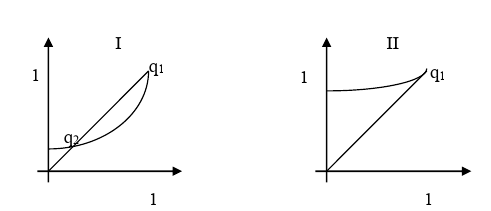
\includegraphics[width=.9\textwidth]{proc_q_vars}
    \caption{Случаи функции $ q $}
    \label{fig:proc_q_vars}
\end{figure}
